\recipe{Creamy Smoky Black Beans}
\label{recipe:creamy_smoky_black_beans}
\makes{4 portions}
\worktime{\SI{30} \minute}
\totaltime{\SI{40} \minute}
\source{Bea}


\begin{ingredients}

\ingroup{For the black beans}
  \item 1 onion, finely chopped
  \item 2 garlic cloves, finely chopped
  \item 30g tomato puree
  \item 1.5 tsp smoked paprika
  \item 240g black beans (cooked)
  \item 50g sour cream
  \item 250g sweetcorn kernels
  \item 100ml water
  \item Oil
  \item Salt
  \item Soy sauce
\ingroup{Toppings} 
  \item pickled red onions
  \item extra sour cream
  \item chopped spring onion
\ingroup{For the pickled red onions}
  \item 1 red onion, finely sliced
  \item 100ml white wine vinegar
\end{ingredients}


\begin{method}
In a large frying pan over a high heat add 1 tbsp of oil than the corn
kernels. Cook until slightly charred. Remove and set aside.

Meanwhile, make the pickled onions by adding the red onion and
white wine vinegar into a small bowl.

Add 1-2 tbsp of oil to the pan then the onion and a pinch of salt. Cook
until softened slightly, about 5 minutes.

Add the garlic, tomato puree and smoked paprika. Cook for 2
minutes.

Add the black beans, sour cream and water. Simmer for a couple of
minutes.

Mash about half the beans to create a creamy texture. Stir to combine.

Stir in half the corn, then taste for seasoning.

Top with the remaining corn, some pickled red onions, chopped
spring onion and extra sour cream. 
  
\end{method}


\begin{figure}[h]
  	\centering
  	
	\begin{tikzpicture}
  		% Save the image in a box to get its dimensions
  		\sbox0{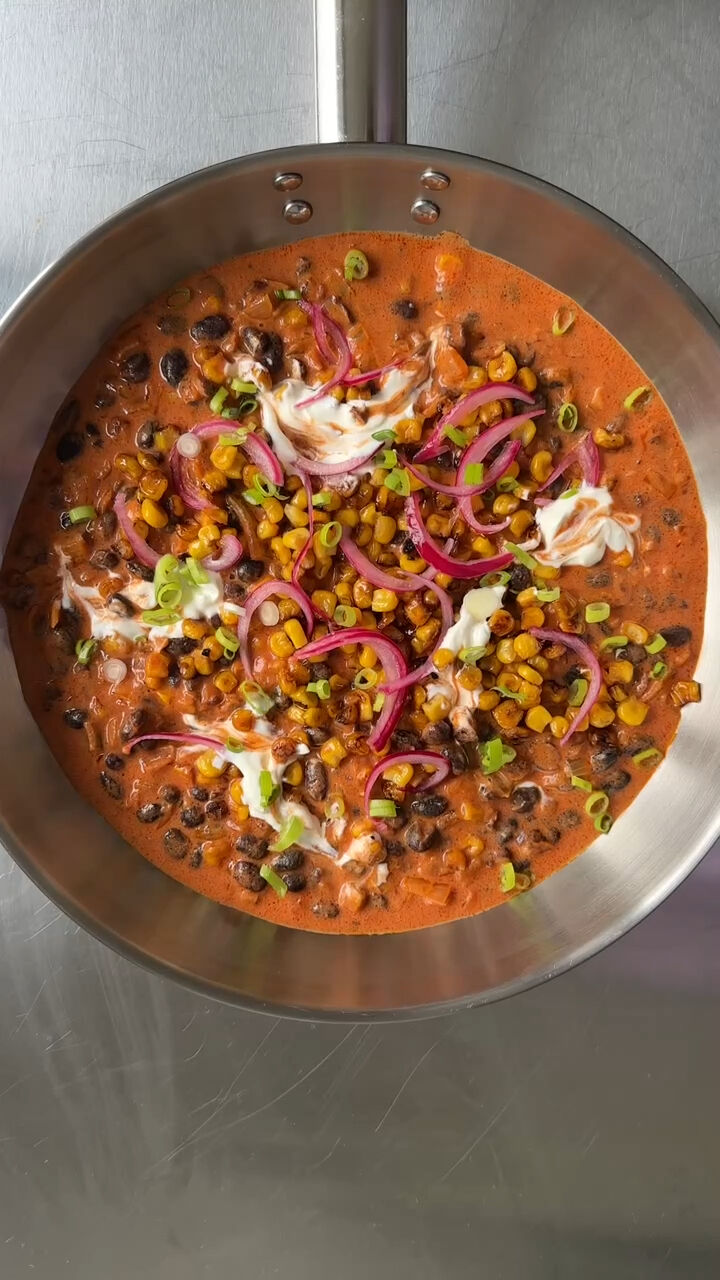
\includegraphics[width = \linewidth]{images/smokyblackbeans.png}}%
  
  		% Draw a clipping rectangle with rounded corners
  		\path[clip, rounded corners=0.5cm] (0,0) rectangle (\wd0,5cm);
  
  		% Place the image inside the clipped area
  		\node[inner sep=0pt, outer sep=0pt, anchor=center] at (0.5\linewidth, 5cm) {\usebox0};
	\end{tikzpicture}

\end{figure}


